	% !TeX spellcheck = en_GB
	\begin{figure}[!htb]
	  \setlength{\unitlength}{\textwidth}
	
	        \begin{picture}(1,0.4)(-0.02,0)
	
	 
	      
	      \put(0.08,0.02){\includegraphics[width=0.75\unitlength]{{./chapter-frequnecy-response/fnp/freq015.eps}}}
	
	      \put(0.47,0.00){\massstiff}
	      
	      
	     
	       \put(0.06,0.235){$\displaystyle\frac{f_{i}}{f}$}
	      
	
	      %\put(0.095,0.218){\small(a)}
	      %\put(0.565,0.218){\small(b)}
	      
	    \end{picture}
	
	  \caption{Frequency ratio as a function of \massstiff. Frequency obtained using QSS simulations, DNS simulations and the linear frequency equation (Eq:\ref{eqn:linear_freq_final})normalised by the undamped natural frequency $f$. $f_{i}$ is the type of frequency i.e. \freqdns,\freqqss ,\freqlin. Data present $\frac{f_{lin}}{f}$ ($\bullet$), $\frac{f_{QSS}}{f}$ (\ding{115}) and $\frac{f_{DNS}}{f}$ ($\times$) at $\massstiff=0.15$, $\reynoldsnumber=200$ and $f=0.025$ }
	    \label{fig:pi2-015-freq}
	\end{figure}
	
	 %vspace{10cm}
